% Delete-min, pass 1: meld adjacent pairs of children.
% Editable source for this diagram. From this directory, regenerate with:
% latex -interaction=nonstopmode -halt-on-error pairing-heap-4.tex
% dvisvgm --no-fonts --exact --bbox=papersize --output=pairing-heap-4.svg pairing-heap-4.dvi
\documentclass[tikz,border=2pt]{standalone}
\usepackage{lmodern}
\usepackage{tikz}
\usetikzlibrary{arrows.meta,backgrounds,shapes.geometric,patterns}
\definecolor{linkred}{HTML}{B5240A}
\definecolor{noteBlue}{HTML}{0067A5}
\definecolor{softgreen}{HTML}{D8EAD0}
\definecolor{softpurple}{HTML}{D9D1E8}
\definecolor{softpink}{HTML}{F5CECF}
\definecolor{softyellow}{HTML}{FFF2C9}
\begin{document}
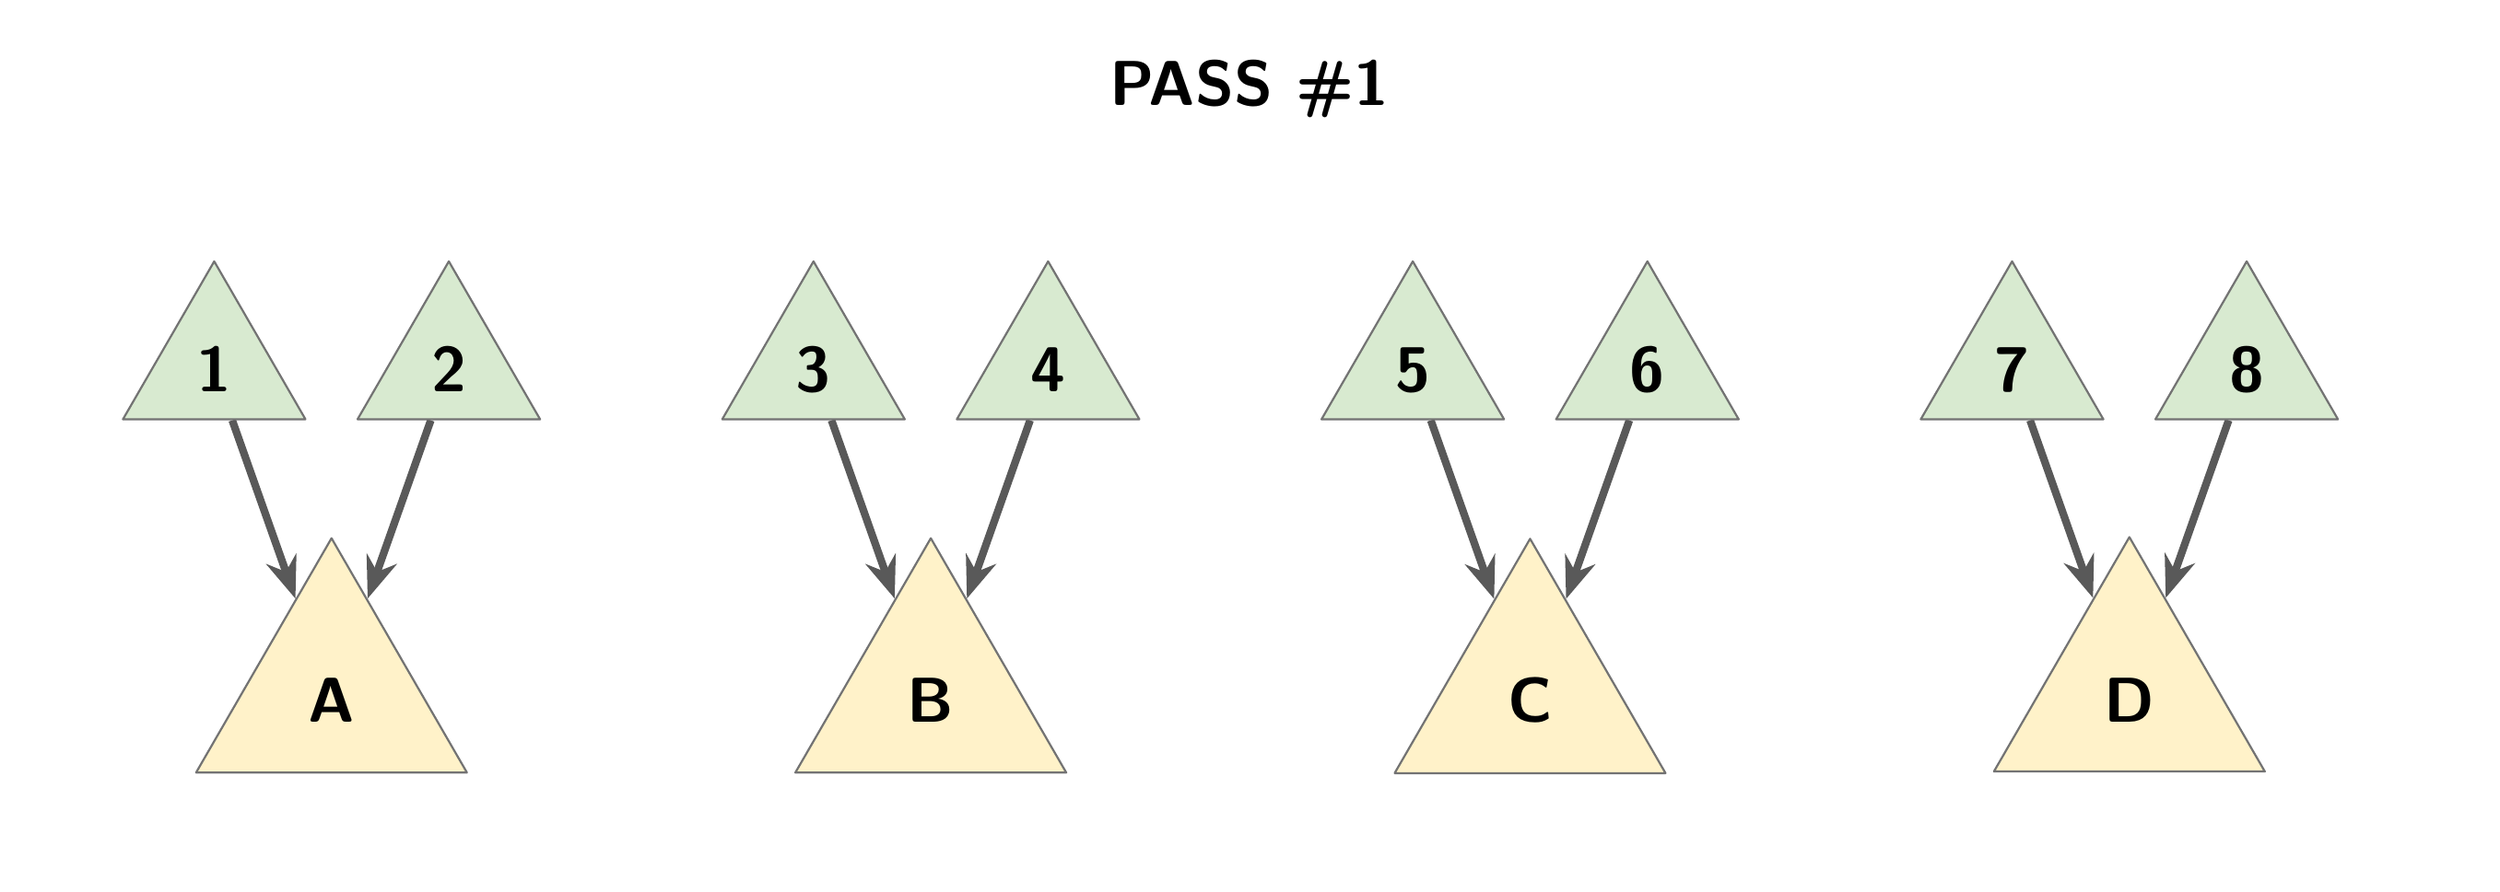
\begin{tikzpicture}[x=1pt,y=-1pt,>=Stealth,line cap=round,line join=round]
\path[use as bounding box] (0,0) rectangle (960,330);
\begin{scope}[on background layer]

\end{scope}
\node[isosceles triangle,draw=black!55,fill=softgreen,text=black,minimum size=62pt,inner sep=0pt,line width=0.8pt,font=\sffamily\fontsize{27}{32.4}\selectfont,shape border rotate=90,isosceles triangle apex angle=60,font=\sffamily\bfseries\fontsize{27}{32}\selectfont] (n00) at (74,135) {1};
\node[isosceles triangle,draw=black!55,fill=softgreen,text=black,minimum size=62pt,inner sep=0pt,line width=0.8pt,font=\sffamily\fontsize{27}{32.4}\selectfont,shape border rotate=90,isosceles triangle apex angle=60,font=\sffamily\bfseries\fontsize{27}{32}\selectfont] (n01) at (166,135) {2};
\node[isosceles triangle,draw=black!55,fill=softyellow,text=black,minimum size=92pt,inner sep=0pt,line width=0.8pt,font=\sffamily\fontsize{27}{32.4}\selectfont,shape border rotate=90,isosceles triangle apex angle=60,font=\sffamily\bfseries\fontsize{27}{32}\selectfont] (m0) at (120,265) {A};
\node[isosceles triangle,draw=black!55,fill=softgreen,text=black,minimum size=62pt,inner sep=0pt,line width=0.8pt,font=\sffamily\fontsize{27}{32.4}\selectfont,shape border rotate=90,isosceles triangle apex angle=60,font=\sffamily\bfseries\fontsize{27}{32}\selectfont] (n10) at (309,135) {3};
\node[isosceles triangle,draw=black!55,fill=softgreen,text=black,minimum size=62pt,inner sep=0pt,line width=0.8pt,font=\sffamily\fontsize{27}{32.4}\selectfont,shape border rotate=90,isosceles triangle apex angle=60,font=\sffamily\bfseries\fontsize{27}{32}\selectfont] (n11) at (401,135) {4};
\node[isosceles triangle,draw=black!55,fill=softyellow,text=black,minimum size=92pt,inner sep=0pt,line width=0.8pt,font=\sffamily\fontsize{27}{32.4}\selectfont,shape border rotate=90,isosceles triangle apex angle=60,font=\sffamily\bfseries\fontsize{27}{32}\selectfont] (m1) at (355,265) {B};
\node[isosceles triangle,draw=black!55,fill=softgreen,text=black,minimum size=62pt,inner sep=0pt,line width=0.8pt,font=\sffamily\fontsize{27}{32.4}\selectfont,shape border rotate=90,isosceles triangle apex angle=60,font=\sffamily\bfseries\fontsize{27}{32}\selectfont] (n20) at (544,135) {5};
\node[isosceles triangle,draw=black!55,fill=softgreen,text=black,minimum size=62pt,inner sep=0pt,line width=0.8pt,font=\sffamily\fontsize{27}{32.4}\selectfont,shape border rotate=90,isosceles triangle apex angle=60,font=\sffamily\bfseries\fontsize{27}{32}\selectfont] (n21) at (636,135) {6};
\node[isosceles triangle,draw=black!55,fill=softyellow,text=black,minimum size=92pt,inner sep=0pt,line width=0.8pt,font=\sffamily\fontsize{27}{32.4}\selectfont,shape border rotate=90,isosceles triangle apex angle=60,font=\sffamily\bfseries\fontsize{27}{32}\selectfont] (m2) at (590,265) {C};
\node[isosceles triangle,draw=black!55,fill=softgreen,text=black,minimum size=62pt,inner sep=0pt,line width=0.8pt,font=\sffamily\fontsize{27}{32.4}\selectfont,shape border rotate=90,isosceles triangle apex angle=60,font=\sffamily\bfseries\fontsize{27}{32}\selectfont] (n30) at (779,135) {7};
\node[isosceles triangle,draw=black!55,fill=softgreen,text=black,minimum size=62pt,inner sep=0pt,line width=0.8pt,font=\sffamily\fontsize{27}{32.4}\selectfont,shape border rotate=90,isosceles triangle apex angle=60,font=\sffamily\bfseries\fontsize{27}{32}\selectfont] (n31) at (871,135) {8};
\node[isosceles triangle,draw=black!55,fill=softyellow,text=black,minimum size=92pt,inner sep=0pt,line width=0.8pt,font=\sffamily\fontsize{27}{32.4}\selectfont,shape border rotate=90,isosceles triangle apex angle=60,font=\sffamily\bfseries\fontsize{27}{32}\selectfont] (m3) at (825,265) {D};
\begin{scope}[on background layer]
\draw[draw=black!65,line width=3pt,->] (n00) -- (m0);
\draw[draw=black!65,line width=3pt,->] (n01) -- (m0);
\draw[draw=black!65,line width=3pt,->] (n10) -- (m1);
\draw[draw=black!65,line width=3pt,->] (n11) -- (m1);
\draw[draw=black!65,line width=3pt,->] (n20) -- (m2);
\draw[draw=black!65,line width=3pt,->] (n21) -- (m2);
\draw[draw=black!65,line width=3pt,->] (n30) -- (m3);
\draw[draw=black!65,line width=3pt,->] (n31) -- (m3);
\end{scope}
\node[anchor=center,text=black,font=\sffamily\fontsize{32}{38.4}\selectfont,font=\sffamily\bfseries\fontsize{32}{38}\selectfont] at (480,25) {PASS \#1};
\end{tikzpicture}
\end{document}
